\begin{figure}[htbp]
\centering
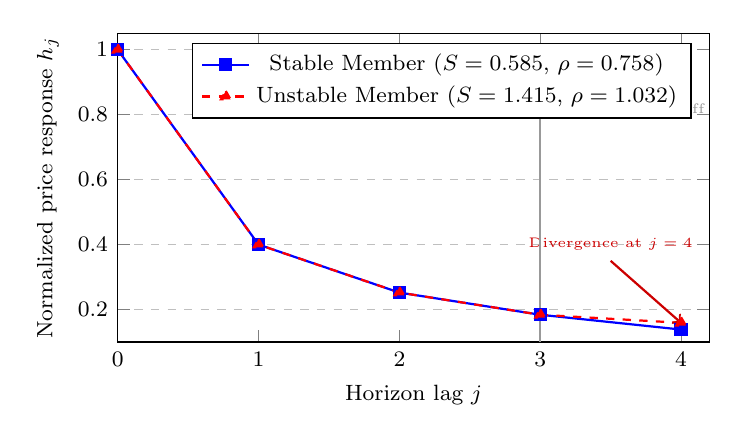
\begin{tikzpicture}
\begin{axis}[
    width=0.75\textwidth,
    height=5.5cm,
    xlabel={Horizon lag $j$},
    ylabel={Normalized price response $h_j$},
    xmin=0, xmax=4.2,
    ymin=0.1, ymax=1.05,
    xtick={0,1,2,3,4},
    legend pos=north east,
    ymajorgrids=true,
    grid style=dashed,
    font=\footnotesize
]
\addplot[color=blue, mark=square*, thick] coordinates {
    (0, 1.0)
    (1, 0.4)
    (2, 0.25230769230769234)
    (3, 0.18400000000000002)
    (4, 0.13842840236686393)
};
\addlegendentry{Stable Member ($S=0.585$, $\rho=0.758$)}

\addplot[color=red, mark=triangle*, thick, dashed] coordinates {
    (0, 1.0)
    (1, 0.4)
    (2, 0.25230769230769234)
    (3, 0.18400000000000002)
    (4, 0.1591976331360947)
};
\addlegendentry{Unstable Member ($S=1.415$, $\rho=1.032$)}

\draw[<-, thick, red!80!black] (axis cs:4, 0.159) -- (axis cs:3.5, 0.35)
    node[above, font=\tiny]{Divergence at $j=4$};
\draw[thick, black!40] (axis cs:3, 0.1) -- (axis cs:3, 1.0)
    node[pos=0.8, right, font=\tiny]{Observation cutoff $H=3$};
\end{axis}
\end{tikzpicture}
\caption{Finite-window ambiguity witness (Table~\ref{tab:retained_witness}): exact overlap of initial price responses ($h_0, \dots, h_3$) between stable ($S < 1$) and unstable ($S > 1$) models.}
\label{fig:F2_finite_window_ambiguity}
\end{figure}
